\documentclass[final]{beamer}

\usepackage[scale=1.24]{beamerposter} % Use the beamerposter package for laying out the poster

\usetheme{confposter} % Use the confposter theme supplied with this template

\setbeamercolor{block title}{fg=ngreen,bg=white} % Colors of the block titles
\setbeamercolor{block body}{fg=black,bg=white} % Colors of the body of blocks
\setbeamercolor{block alerted title}{fg=white,bg=dblue!70} % Colors of the highlighted block titles
\setbeamercolor{block alerted body}{fg=black,bg=dblue!10} % Colors of the body of highlighted blocks
% Many more colors are available for use in beamerthemeconfposter.sty

%-----------------------------------------------------------
% Define the column widths and overall poster size
% To set effective sepwid, onecolwid and twocolwid values, first choose how many columns you want and how much separation you want between columns
% In this template, the separation width chosen is 0.024 of the paper width and a 4-column layout
% onecolwid should therefore be (1-(# of columns+1)*sepwid)/# of columns e.g. (1-(4+1)*0.024)/4 = 0.22
% Set twocolwid to be (2*onecolwid)+sepwid = 0.464
% Set threecolwid to be (3*onecolwid)+2*sepwid = 0.708

\newlength{\sepwid}
\newlength{\onecolwid}
\newlength{\twocolwid}
\newlength{\threecolwid}
\setlength{\paperwidth}{48in} % A0 width: 46.8in
\setlength{\paperheight}{36in} % A0 height: 33.1in
\setlength{\sepwid}{0.024\paperwidth} % Separation width (white space) between columns
\setlength{\onecolwid}{0.22\paperwidth} % Width of one column
\setlength{\twocolwid}{0.464\paperwidth} % Width of two columns
\setlength{\threecolwid}{0.708\paperwidth} % Width of three columns
\setlength{\topmargin}{-0.5in} % Reduce the top margin size
%-----------------------------------------------------------

\usepackage{graphicx}  % Required for including images

\usepackage{booktabs} % Top and bottom rules for tables
%----------------------------------------------------------------------------------------
%	TITLE SECTION
%----------------------------------------------------------------------------------------

\title{Bayesian Spatial Relationsip Between Kaitz Index and PR Emplyment} % Poster title

\author{Alejandro M. Ouslan and Julio C. Hernandez} % Author(s)

\institute{Department of Mathematics from the University of Puerto Rico Mayaguez} % Institution(s)

%----------------------------------------------------------------------------------------

\begin{document}

\addtobeamertemplate{block end}{}{\vspace*{2ex}} % White space under blocks
\addtobeamertemplate{block alerted end}{}{\vspace*{2ex}} % White space under highlighted (alert) blocks

\setlength{\belowcaptionskip}{2ex} % White space under figures
\setlength\belowdisplayshortskip{2ex} % White space under equations

\begin{frame}[t] % The whole poster is enclosed in one beamer frame

	\begin{columns}[t] % The whole poster consists of three major columns, the second of which is split into two columns twice - the [t] option aligns each column's content to the top

		\begin{column}{\sepwid}\end{column} % Empty spacer column

		\begin{column}{\onecolwid} % The first column

			%----------------------------------------------------------------------------------------
			%	INTRODUCTION
			%----------------------------------------------------------------------------------------

			\begin{block}{Introduction}

				There are many studies looking at the impact of minimum salarie on the employment but there are not many studies at looking the spatial effect in the changes
				in the minimum salaries. Throught this studies used the Kaitz index to measure the effects of mimnume salarieis in all the zipcodes of PR. We found there
				is a negative "spill-over" effect of the Kaitz index on employment


			\end{block}

			%------------------------------------------------

			\begin{figure}
				
\includegraphics[width=0.8\linewidth]{placeholder.jpg}
				\caption{Figure caption}
			\end{figure}
			\begin{block}{Materials}

				The following materials were required to complete the research:

				\begin{itemize}
					\item Curabitur pellentesque dignissim
					\item Eu facilisis est tempus quis
					\item Duis porta consequat lorem
					\item Eu facilisis est tempus quis
				\end{itemize}

				The materials were prepared according to the steps outlined below:

				\begin{enumerate}
					\item Curabitur pellentesque dignissim
					\item Eu facilisis est tempus quis
					\item Duis porta consequat lorem
					\item Curabitur pellentesque dignissim
				\end{enumerate}

			\end{block}

			%----------------------------------------------------------------------------------------

		\end{column} % End of the first column

		\begin{column}{\sepwid}\end{column} % Empty spacer column

		\begin{column}{\twocolwid} % Begin a column which is two columns wide (column 2)

			\begin{columns}[t,totalwidth=\twocolwid] % Split up the two columns wide column

				\begin{column}{\onecolwid}\vspace{-.6in} % The first column within column 2 (column 2.1)


					%----------------------------------------------------------------------------------------

				\end{column} % End of column 2.1

				\begin{column}{\onecolwid}\vspace{-.6in} % The second column within column 2 (column 2.2)

					%----------------------------------------------------------------------------------------
					%	METHODS
					%----------------------------------------------------------------------------------------

					\begin{block}{Data methods}

						For this study we desided to use a Bayesian apraach to estimate the spill-over effects in witch we specified weakly informative priors for all model terms,
						by loosely scaling them to the observed data and used a tune of 2000 samples and a target accept of $.95$
						\begin{figure}
							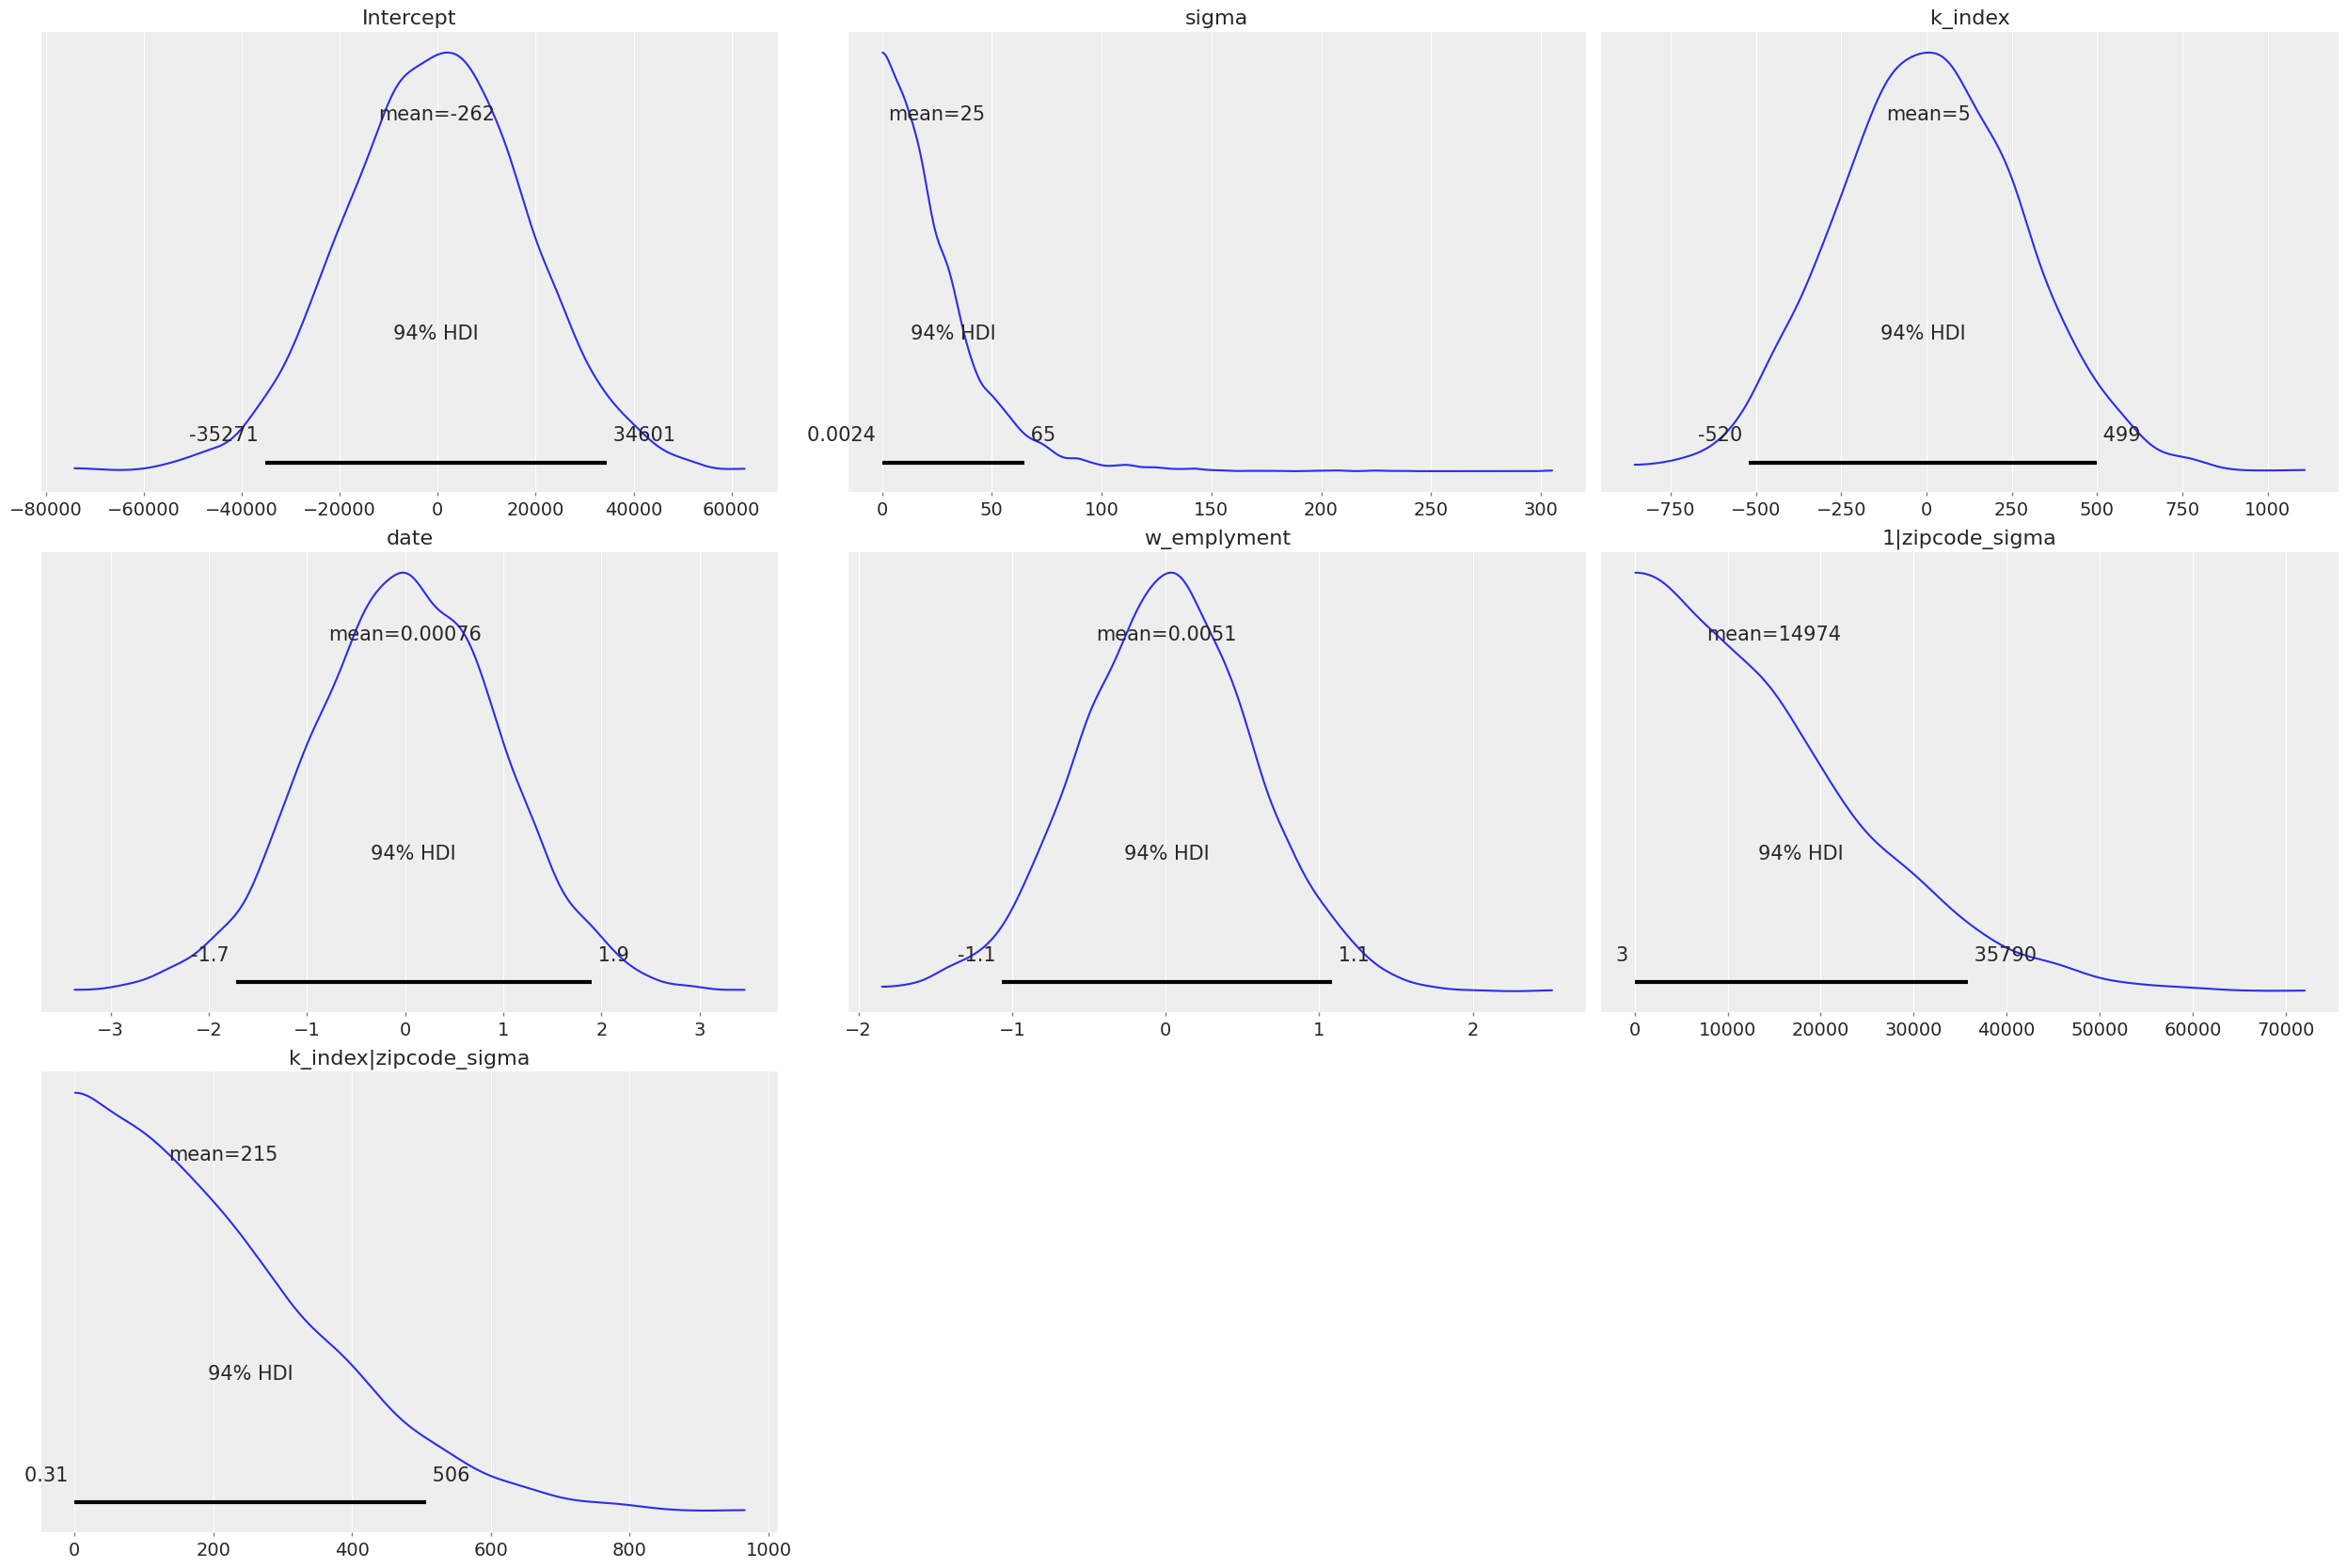
\includegraphics[width=0.8\linewidth]{priori.png}
							\caption{Figure caption}
						\end{figure}
					\end{block}

					%----------------------------------------------------------------------------------------

				\end{column} % End of column 2.2

			\end{columns} % End of the split of column 2 - any content after this will now take up 2 columns width



			%----------------------------------------------------------------------------------------

			\begin{columns}[t,totalwidth=\twocolwid] % Split up the two columns wide column again

				\begin{column}{\onecolwid} % The first column within column 2 (column 2.1)

					%----------------------------------------------------------------------------------------
					%	MATHEMATICAL SECTION
					%----------------------------------------------------------------------------------------

					\begin{block}{Mathematical Section}

						The main coefficient for this study is the \textbf{Kaitz Indez} \cite{baker1994demography}. The idez is calculated as follows:
						\begin{equation}
							Kaitz = \frac{m}{w}
						\end{equation}

						where $m$ represents the nomiinal legal wage, and $w$ is the mean wage. To account fo the spatial autocorrelation, the Kaitz index is modified as:

						\begin{equation}
							Kaitz_{it} = \frac{m_t}{\bar{w}_{it}}
						\end{equation}

						where $m_t$ is the minimum wage for the specific time period, and $\bar{w}_{it}$ is the mean wage for the $i$-th zipcode at time $t$.

						To asses teh impact of the Kaitz index and its spillover effects, follow the following model according to the speciifications in \cite{elhorst2003specification}
						\begin{equation}
							y_{it} = \rho \sum_{j=1}^N w_{ij} y_{jt}  +  Kaitz_{it} \cdot \beta  +  \mu_i  +  e_{it}
						\end{equation}
						Where $\sum_{j=1}^N w_{ij} y_{jt}$ represents the mean Emplyment of the neighbors of zipcode $i$. $\rho$ is the spillover effect, $\mu_i$ is the spatial error and $\epsilon_{it}$ is the error term
					\end{block}

					%----------------------------------------------------------------------------------------

				\end{column} % End of column 2.1

				\begin{column}{\onecolwid} % The second column within column 2 (column 2.2)

					%----------------------------------------------------------------------------------------
					%	RESULTS
					%----------------------------------------------------------------------------------------

					\begin{block}{Results}

						\begin{figure}
							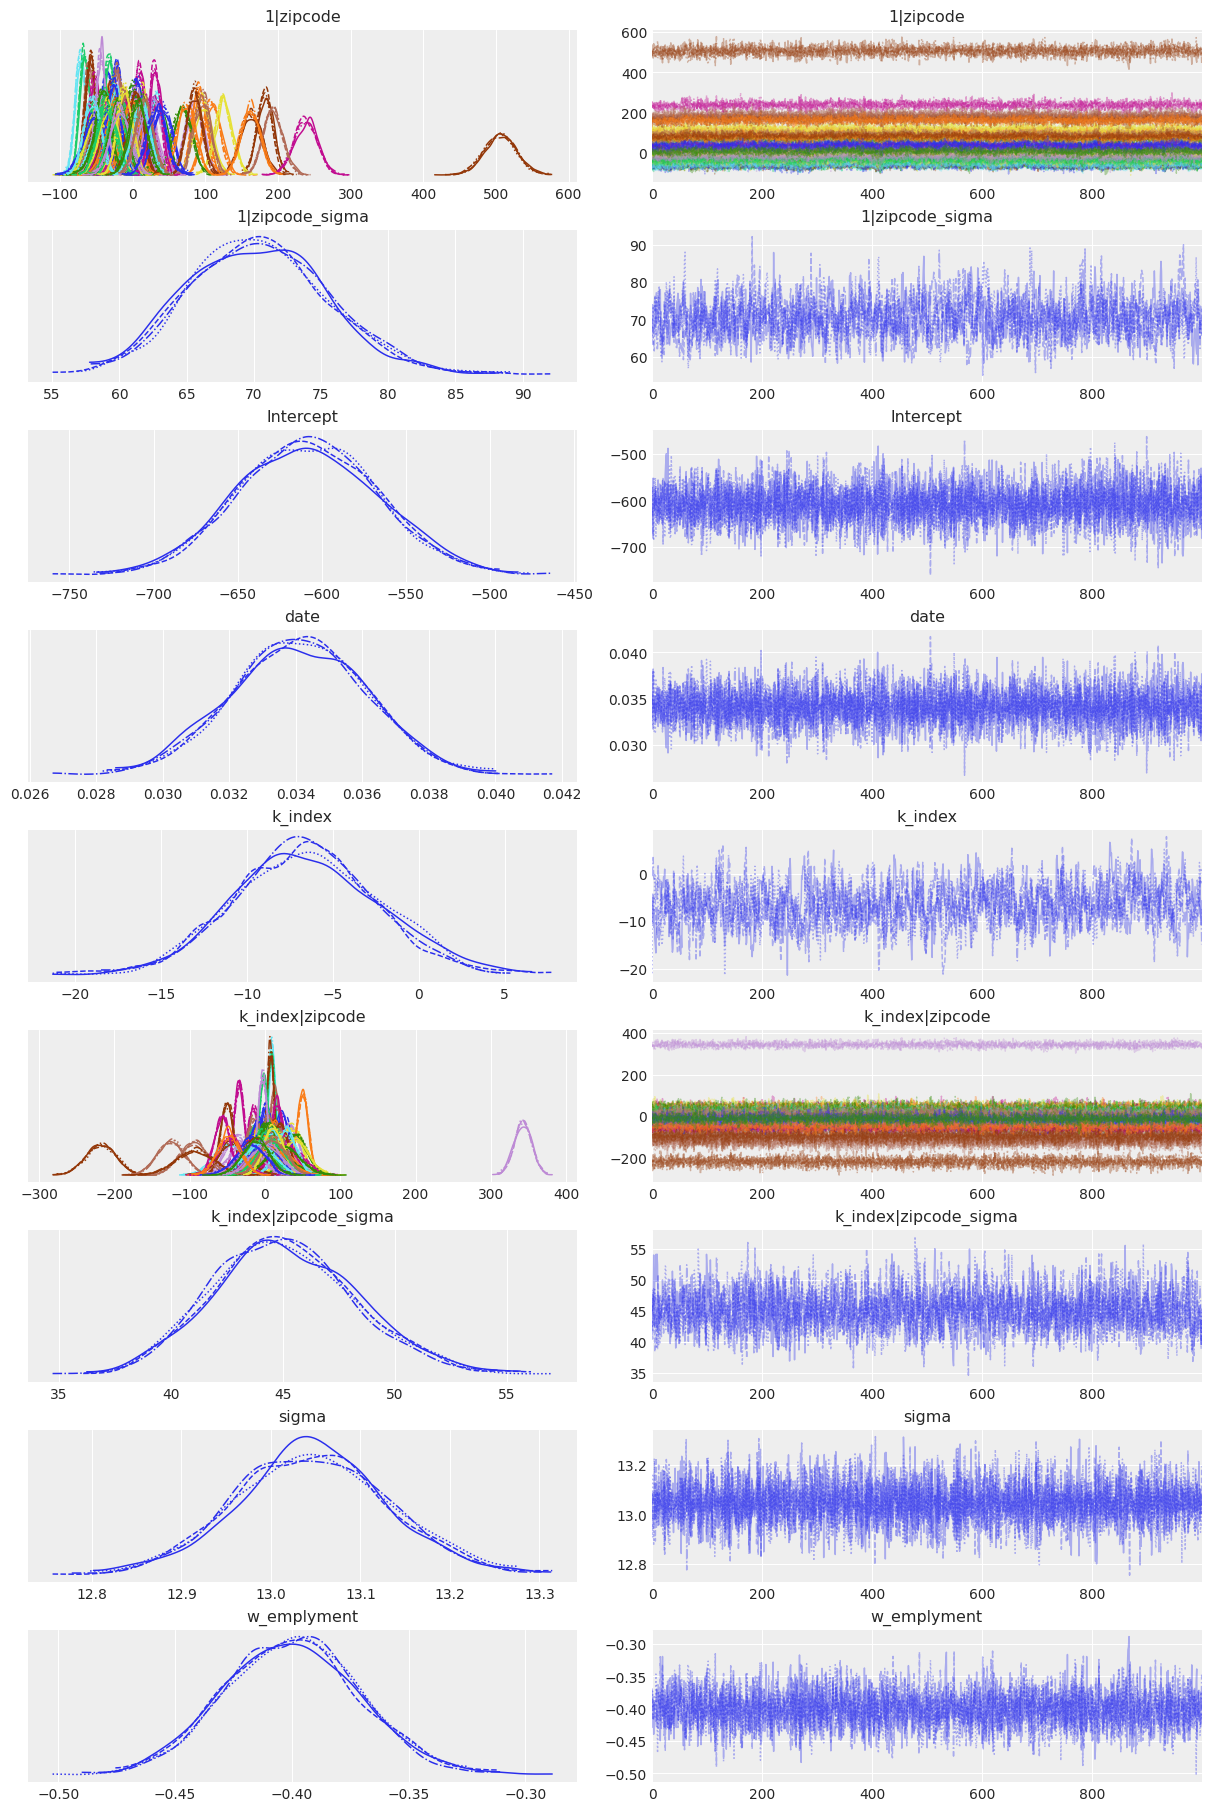
\includegraphics[width=0.8\linewidth]{results.png}
							\caption{Figure caption}
						\end{figure}

						Nunc tempus venenatis facilisis. Curabitur suscipit consequat eros non porttitor. Sed a massa dolor, id ornare enim:

						\begin{table}
							\vspace{2ex}
							\begin{tabular}{l l l}
								\toprule
								\textbf{Treatments} & \textbf{Response 1} & \textbf{Response 2} \\
								\midrule
								Treatment 1         & 0.0003262           & 0.562               \\
								Treatment 2         & 0.0015681           & 0.910               \\
								Treatment 3         & 0.0009271           & 0.296               \\
								\bottomrule
							\end{tabular}
							\caption{Table caption}
						\end{table}

					\end{block}

					%----------------------------------------------------------------------------------------

				\end{column} % End of column 2.2

			\end{columns} % End of the split of column 2

		\end{column} % End of the second column

		\begin{column}{\sepwid}\end{column} % Empty spacer column

		\begin{column}{\onecolwid} % The third column

			%----------------------------------------------------------------------------------------
			%	CONCLUSION
			%----------------------------------------------------------------------------------------

			\begin{block}{Conclusion}

				Nunc tempus venenatis facilisis. \textbf{Curabitur suscipit} consequat eros non porttitor. Sed a massa dolor, id ornare enim. Fusce quis massa dictum tortor \textbf{tincidunt mattis}. Donec quam est, lobortis quis pretium at, laoreet scelerisque lacus. Nam quis odio enim, in molestie libero. Vivamus cursus mi at \textit{nulla elementum sollicitudin}.

			\end{block}


			%----------------------------------------------------------------------------------------
			%	REFERENCES
			%----------------------------------------------------------------------------------------

			\begin{block}{References}

				\nocite{*} % Insert publications even if they are not cited in the poster
				\small{\bibliographystyle{unsrt}
					\bibliography{references}\vspace{0.75in}}

			\end{block}

			%----------------------------------------------------------------------------------------
			%	ACKNOWLEDGEMENTS
			%----------------------------------------------------------------------------------------

			\setbeamercolor{block title}{fg=red,bg=white} % Change the block title color

			\begin{block}{Acknowledgements}

				\small{\rmfamily{Nam mollis tristique neque eu luctus. Suspendisse rutrum congue nisi sed convallis. Aenean id neque dolor. Pellentesque habitant morbi tristique senectus et netus et malesuada fames ac turpis egestas.}} \\

			\end{block}

			%----------------------------------------------------------------------------------------
			%	CONTACT INFORMATION
			%----------------------------------------------------------------------------------------

			\setbeamercolor{block alerted title}{fg=black,bg=norange} % Change the alert block title colors
			\setbeamercolor{block alerted body}{fg=black,bg=white} % Change the alert block body colors

			\begin{alertblock}{Contact Information}

				\begin{itemize}
					\item Web: \href{http://www.university.edu/smithlab}{http://www.university.edu/smithlab}
					\item Email: \href{mailto:john@smith.com}{john@smith.com}
					\item Phone: +1 (000) 111 1111
				\end{itemize}

			\end{alertblock}

			\begin{center}
				\begin{tabular}{ccc}
					
\includegraphics[width=0.4\linewidth]{logo.png} & \hfill & 
\includegraphics[width=0.4\linewidth]{logo.png}
				\end{tabular}
			\end{center}

			%----------------------------------------------------------------------------------------

		\end{column} % End of the third column

	\end{columns} % End of all the columns in the poster

\end{frame} % End of the enclosing frame

\end{document}
